% Notes for students: the logistic regression lecture, step by step.
% Every number in these notes is computed by check_notes.py (same folder).
% Build:  latexmk -pdf logistic_regression_notes.tex
\documentclass[11pt]{article}
\usepackage[margin=1in]{geometry}
\usepackage[T1]{fontenc}
\usepackage{lmodern}
\usepackage{amsmath,amssymb}
\usepackage{booktabs}
\usepackage{array}
\usepackage{xcolor}
\usepackage{float}
\usepackage{pgfplots}
\pgfplotsset{compat=1.17}
\usepackage[hidelinks]{hyperref}
\usepackage{microtype}
\setlength{\parindent}{0pt}
\setlength{\parskip}{0.6em}

\definecolor{zeroone}{HTML}{D9541E}   % orange, as on the slides
\definecolor{hingec}{HTML}{0E8C8C}    % teal
\definecolor{logc}{HTML}{B7860B}      % amber

\newcommand{\ind}[1]{\mathbf{1}\bigl[#1\bigr]}
\newcommand{\Loss}{\mathcal{L}}

\title{Logistic regression, step by step\\[0.3em]\large Notes to go with the lecture slides}
\author{}
\date{}

\begin{document}
\maketitle

These notes go through the logistic regression lecture slowly. They follow the order of the slides
and fill in the steps that the slides skip. Section~\ref{sec:zeroone}, on the 0--1 loss, is the
longest, because it is where the rest of the lecture starts. If a formula on the slides looked like
it came out of nowhere, its derivation should be here.

You need only a little algebra: adding up a list of numbers, the exponential function $e^z$, and the
natural logarithm $\log$. The rules for $e$ and $\log$ that we use are collected in
Appendix~\ref{app:rules}.

\tableofcontents

%======================================================================
\section{What training means}
%======================================================================

\subsection*{The data}

We have $n$ training examples. Example number $i$ has an input $x_i$ and a label $y_i$. In this
lecture there are two classes, and we write the labels as numbers:
\[
  y_i = +1 \ \text{(the positive class)} \qquad\text{or}\qquad y_i = -1 \ \text{(the negative class)}.
\]
The labels could have been called ``pass'' and ``fail'', or 1 and 0. We use $+1$ and $-1$ because it
makes the formulas in Section~\ref{sec:zeroone} short. We write the whole training set as
$D = \{(x_1, y_1), \dots, (x_n, y_n)\}$, or $D = \{(x_i, y_i)\}$ for short.

\subsection*{The model}

A model is a formula that turns an input into a prediction. It has some numbers in it, the
parameters, that training has to choose. We collect the parameters in one symbol, $\theta$ (theta),
and write the prediction for example $i$ as
\[
  \hat y_i = f(x_i \mid \theta).
\]
The hat on $\hat y_i$ means ``predicted'', as opposed to the true label $y_i$. The bar in
$f(x_i \mid \theta)$ is read ``given'': the prediction depends on the input, once the parameters are
fixed.

The model for the whole lecture is the linear score
\[
  f(x) = w \cdot x + b .
\]
With one input feature, $w \cdot x$ is just $w$ times $x$. With several features
$x = (x_1, \dots, x_d)$ it is $w_1 x_1 + \dots + w_d x_d$. The parameters are $\theta = (w, b)$.
This is the same score the linear SVM uses.

\subsection*{The loss}

A loss is a number that says how badly a choice of parameters fits the training data. Training means
finding the parameters with the smallest loss:
\[
  \min_\theta \; \Loss(\theta; D).
\]
Read this as: ``over all choices of $\theta$, make $\Loss$ as small as possible.'' Methods differ in
their model and in their loss. Linear regression, for example, adds up squared errors,
\[
  \Loss = \sum_i (y_i - \hat y_i)^2 .
\]
The symbol $\sum_i$ means ``add up over all examples $i = 1, \dots, n$''. With three examples,
$\sum_i (y_i - \hat y_i)^2$ is $(y_1 - \hat y_1)^2 + (y_2 - \hat y_2)^2 + (y_3 - \hat y_3)^2$.

The question for this lecture is: what loss should a classifier use?

%======================================================================
\section{Counting mistakes: the 0--1 loss}\label{sec:zeroone}
%======================================================================

The most natural loss for a classifier is the number of training examples it gets wrong. This section
builds a formula for that number, one step at a time.

\subsection{Two conditions}

A score $f(x)$ is turned into a class by comparing it with a threshold $t$: predict $+1$ when the
score is above $t$, and $-1$ when it is below. So we want
\begin{align*}
  f(x_i) &> t \quad \text{for every example with } y_i = +1, \\
  f(x_i) &< t \quad \text{for every example with } y_i = -1.
\end{align*}
Positives should score above the threshold, negatives below it. This is the same picture as in the
ROC lecture. Each example either meets its condition (a correct prediction) or breaks it (a mistake).
The four possibilities are the four cells of the table on the slide:

\begin{center}
\begin{tabular}{lcc}
  \toprule
  & predicted $+1$ & predicted $-1$ \\
  \midrule
  true label $+1$ & correct & mistake \\
  true label $-1$ & mistake & correct \\
  \bottomrule
\end{tabular}
\end{center}

The training error is the number of examples that break their condition. To write it as a formula we
first turn the two conditions into one.

\subsection{Choose the threshold 0}

For a score like $w \cdot x + b$ the usual threshold is $t = 0$. This loses nothing: a threshold
$t \ne 0$ can be moved into the score by changing $b$ to $b - t$, because $w \cdot x + b > t$ says
the same as $w \cdot x + (b - t) > 0$. (If $f$ is a probability, the usual threshold is 0.5. We will
see in Section~\ref{sec:predict} that for logistic regression ``probability above 0.5'' and ``score
above 0'' are the same thing.)

With $t = 0$ the two conditions read
\begin{align*}
  f(x_i) &> 0 \quad \text{if } y_i = +1, \\
  f(x_i) &< 0 \quad \text{if } y_i = -1.
\end{align*}

\subsection{From two conditions to one: multiply by the label}

Here is the step that the slide does in one line. Look at the product $y_i f(x_i)$ of the label and
the score.
\begin{itemize}
  \item If $y_i = +1$, then $y_i f(x_i) = f(x_i)$. The condition $f(x_i) > 0$ is the same as
        $y_i f(x_i) > 0$.
  \item If $y_i = -1$, then $y_i f(x_i) = -f(x_i)$. The condition $f(x_i) < 0$ is the same as
        $-f(x_i) > 0$, because multiplying both sides of an inequality by $-1$ flips it. So it too is
        the same as $y_i f(x_i) > 0$.
\end{itemize}
Both conditions have become one:
\[
  \boxed{\;y_i f(x_i) > 0 \quad\text{means example } i \text{ is classified correctly.}\;}
\]
The table below checks all four cases. The sign of the score is the prediction; the sign of the
product says whether the prediction was right.

\begin{center}
\begin{tabular}{cccc}
  \toprule
  label $y_i$ & sign of the score $f(x_i)$ & sign of $y_i f(x_i)$ & result \\
  \midrule
  $+1$ & $+$ & $+$ & correct \\
  $+1$ & $-$ & $-$ & mistake \\
  $-1$ & $-$ & $+$ & correct \\
  $-1$ & $+$ & $-$ & mistake \\
  \bottomrule
\end{tabular}
\end{center}

This works only because we chose the labels $+1$ and $-1$. Multiplying by $+1$ leaves the score
alone; multiplying by $-1$ flips its sign, which turns ``should be negative'' into ``should be
positive''.

\subsection{A mistake is $y_i f(x_i) \le 0$}

The opposite of $y_i f(x_i) > 0$ is $y_i f(x_i) \le 0$. So example $i$ is a mistake when
$y_i f(x_i) \le 0$. The case $y_i f(x_i) = 0$ means the score is exactly 0: the point sits on the
boundary and the classifier cannot decide. Counting it as a mistake is a convention.

\subsection{The indicator function}

To count mistakes with a formula, we need something that is 1 for a mistake and 0 for a correct
example. That is the indicator function. For any statement $A$,
\[
  \ind{A} =
  \begin{cases}
    1 & \text{if } A \text{ is true}, \\
    0 & \text{if } A \text{ is false}.
  \end{cases}
\]
Some examples: $\ind{3 > 2} = 1$, $\ind{2 > 3} = 0$, $\ind{-0.5 \le 0} = 1$, $\ind{1.5 \le 0} = 0$.
Some books write it as $\mathbb{1}[A]$ or $I(A)$; it is the same thing.

\subsection{Adding up: the 0--1 loss}

The cost of example $i$ is $\ind{y_i f(x_i) \le 0}$: 1 for a mistake, 0 for a correct prediction.
Adding up over all examples counts the mistakes:
\[
  \boxed{\;\Loss_{0\text{--}1} = \sum_i \ind{y_i f(x_i) \le 0} = \text{number of training mistakes.}\;}
\]
It is called the 0--1 loss because each example costs either 0 or 1. Dividing by $n$ gives the
fraction of mistakes, the training error rate.

\paragraph{Worked example.} Five training examples with these labels and scores:

\begin{center}
\begin{tabular}{cccccc}
  \toprule
  $i$ & $y_i$ & $f(x_i)$ & $y_i f(x_i)$ & correct? & $\ind{y_i f(x_i) \le 0}$ \\
  \midrule
  1 & $+1$ & $+2.0$ & $+2.0$ & yes & 0 \\
  2 & $+1$ & $-0.5$ & $-0.5$ & no  & 1 \\
  3 & $-1$ & $-1.5$ & $+1.5$ & yes & 0 \\
  4 & $-1$ & $+0.8$ & $-0.8$ & no  & 1 \\
  5 & $+1$ & $+0.3$ & $+0.3$ & yes & 0 \\
  \midrule
  \multicolumn{5}{r}{$\Loss_{0\text{--}1}$ (sum of the last column)} & 2 \\
  \bottomrule
\end{tabular}
\end{center}

Example 3 shows the trick at work: its score is negative, but so is its label, so the product is
positive and the prediction is correct. Two of the five examples are mistakes, an error rate of 40\%.
We will reuse these five examples for the other two losses.

\subsection{The margin $m = y f(x)$}

The product $y f(x)$ will appear in every loss from now on, so it gets a name here: the margin of an
example, $m = y f(x)$. (The SVM's margin, the width of the band around the line, is a related but
different quantity.) Its sign says whether the example is classified correctly. Its size says how
far the score is from the boundary: a large positive $m$ is a confident correct prediction, a large
negative $m$ is a confident mistake.

On the slides, the loss plots use $m = y f(x)$ as the horizontal axis. As a function of $m$, the 0--1
loss is a step: 1 for $m \le 0$ and 0 for $m > 0$ (the orange line in Figure~\ref{fig:losses}).

\subsection{Why not minimize the 0--1 loss directly?}

It is the loss we care about, so why not train with it? There are three reasons.

\begin{enumerate}
  \item It gives no direction. A small change to $w$ or $b$ usually changes no prediction at all, so
        the count stays the same; then, when a point crosses the boundary, it jumps by 1. A method
        that improves the parameters by following the slope of the loss (next week: gradient
        descent) finds no slope to follow. For example, in the hours-of-study data on the slides
        (Section~\ref{sec:predict}), the fitted boundary is at 5.40 hours and the nearest training
        points are at 5.3 and 5.6 hours. Any boundary between those two gives the same 6 mistakes.
  \item It is hard to minimize. Finding the line with the fewest training mistakes is NP-hard in
        general, as the number of features grows (Ben-David, Eiron and Long, 2003): no efficient
        method is known.
  \item It has no preference among lines with the same count. A line that barely separates the
        classes and one with a wide margin cost the same.
\end{enumerate}

So we use a stand-in: a loss that is easy to minimize and still punishes mistakes. The SVM uses the
hinge loss, logistic regression uses the log loss.

%======================================================================
\section{The SVM as a loss: the hinge}\label{sec:hinge}
%======================================================================

The hinge loss of one example with margin $m = y f(x)$ is
\[
  \max(0,\, 1 - m) =
  \begin{cases}
    0     & \text{if } m \ge 1, \\
    1 - m & \text{if } m < 1 .
  \end{cases}
\]
Here $\max(a, b)$ is the larger of the two numbers. An example with margin at least 1 pays nothing.
Below 1, the cost grows by 1 for each unit of margin: $m = 0.5$ costs 0.5, $m = 0$ costs 1,
$m = -1$ costs 2, $m = -2$ costs 3. So mistakes cost more the further they are on the wrong side,
and even correct examples pay a little if they are too close to the boundary ($0 < m < 1$).

The soft-margin SVM minimizes
\[
  \Loss = \tfrac12 \|w\|^2 + C \sum_i \max\bigl(0,\, 1 - y_i f(x_i)\bigr).
\]
The first term keeps $w$ small, which makes the margin wide; $\|w\|^2 = w_1^2 + \dots + w_d^2$. The
second term is the total hinge loss, and $C$ sets how much it counts compared with the first. At the
solution, the slack $\xi_i$ of the SVM lecture equals the hinge loss of example $i$, so this is the
same problem as $\tfrac12 \|w\|^2 + C \sum_i \xi_i$.

\paragraph{Worked example.} For the five examples above, the hinge losses are 0, 1.5, 0, 1.8 and 0.7,
a total of 4.0. Example 5 is classified correctly ($m = 0.3$) but still pays 0.7, because it is inside
the margin.

%======================================================================
\section{Same score, another loss: the log loss}\label{sec:log}
%======================================================================

Logistic regression replaces the hinge with the log loss,
\[
  \log\bigl(1 + e^{-m}\bigr), \qquad m = y f(x).
\]
Here $\log$ is the natural logarithm. Some values:

\begin{center}
\begin{tabular}{rccccccc}
  \toprule
  margin $m$ & $-2$ & $-1$ & $0$ & $0.5$ & $1$ & $2$ & $4$ \\
  \midrule
  0--1 loss      & 1     & 1     & 1     & 0     & 0     & 0     & 0 \\
  hinge loss     & 3     & 2     & 1     & 0.5   & 0     & 0     & 0 \\
  log loss       & 2.127 & 1.313 & 0.693 & 0.474 & 0.313 & 0.127 & 0.018 \\
  \bottomrule
\end{tabular}
\end{center}


Three things to notice, comparing with the hinge (Figure~\ref{fig:losses}):
\begin{itemize}
  \item The log loss is never exactly zero. Even a confidently correct example pays a little, so every
        example has some say in where the boundary goes, not only the ones near it.
  \item Far on the wrong side it grows linearly, like the hinge. For very negative $m$, $e^{-m}$ is
        huge, the 1 hardly matters, and $\log(1 + e^{-m}) \approx \log(e^{-m}) = -m$. For example, at
        $m = -5$ the log loss is 5.007.
  \item It is smooth: no corner at $m = 1$.
\end{itemize}

\begin{figure}[H]
\centering
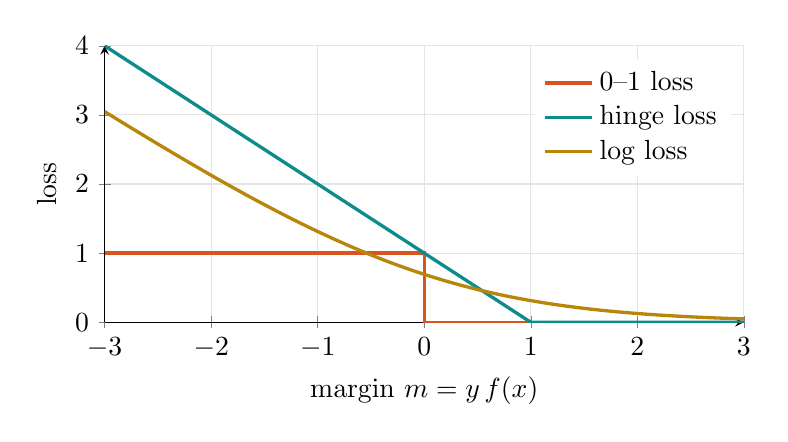
\begin{tikzpicture}
\begin{axis}[width=0.8\textwidth, height=0.42\textwidth, xmin=-3, xmax=3, ymin=0, ymax=4, xtick={-3,...,3},
  xlabel={margin $m = y\,f(x)$}, ylabel={loss}, axis lines=left, grid=major, grid style={gray!20},
  legend style={draw=none, at={(0.98,0.95)}, anchor=north east}, legend cell align=left]
  \addplot[zeroone, very thick, const plot] coordinates {(-3,1) (0,1) (0,0) (3,0)};
  \addlegendentry{0--1 loss}
  \addplot[hingec, very thick, domain=-3:3, samples=7] {max(0, 1 - x)};
  \addlegendentry{hinge loss}
  \addplot[logc, very thick, domain=-3:3, samples=120] {ln(1 + exp(-x))};
  \addlegendentry{log loss}
\end{axis}
\end{tikzpicture}
\caption{The three losses as functions of the margin $m = y f(x)$. Positive $m$ means a correct
prediction. Unlike the 0--1 loss, the hinge and the log loss have a slope that points towards fewer
mistakes, and both are convex (bowl-shaped), which makes them easy to minimize.}
\label{fig:losses}
\end{figure}

Logistic regression minimizes the same kind of objective as the SVM, with the log loss in place of
the hinge:
\[
  \Loss = \tfrac12 \|w\|^2 + C \sum_i \log\bigl(1 + e^{-y_i f(x_i)}\bigr).
\]
This is what scikit-learn's \texttt{LogisticRegression} minimizes (it does not penalize $b$).

\paragraph{Worked example.} For the five examples, the log losses are 0.127, 0.974, 0.201, 1.171 and
0.554, a total of 3.028.

So far the log loss is just another curve. The next two sections show where it comes from.

%======================================================================
\section{From score to probability: the sigmoid}\label{sec:sigmoid}
%======================================================================

The sigmoid function squashes any number into the interval between 0 and 1:
\[
  \sigma(z) = \frac{1}{1 + e^{-z}} .
\]
At $z = 0$, $e^{0} = 1$ and $\sigma(0) = 1/2$. For large positive $z$, $e^{-z}$ is close to 0 and
$\sigma(z)$ is close to 1. For large negative $z$, $e^{-z}$ is huge and $\sigma(z)$ is close to 0. In
between it rises smoothly: $\sigma(-2) = 0.12$, $\sigma(0) = 0.5$, $\sigma(2) = 0.88$.

Logistic regression reads the score as a probability:
\[
  p(y = +1 \mid x) = \sigma\bigl(f(x)\bigr) = \frac{1}{1 + e^{-(w \cdot x + b)}} .
\]
The score is the same as before. The sigmoid changes how we read it, not where the boundary is.

\subsection*{The probability of the true class is $\sigma(y f)$}

Write $f$ for the score $f(x)$. The probability of the negative class is what is left over:
\begin{align*}
  p(y = -1 \mid x) &= 1 - \sigma(f) \\
    &= 1 - \frac{1}{1 + e^{-f}}
     = \frac{(1 + e^{-f}) - 1}{1 + e^{-f}}
     = \frac{e^{-f}}{1 + e^{-f}} && \text{(common denominator)} \\
    &= \frac{e^{-f} \cdot e^{f}}{(1 + e^{-f}) \cdot e^{f}}
     = \frac{1}{e^{f} + 1} && \text{(multiply top and bottom by } e^{f}\text{)} \\
    &= \sigma(-f) && \text{(the definition of } \sigma \text{ with } z = -f\text{)}.
\end{align*}
So $p(y = +1 \mid x) = \sigma(f)$ and $p(y = -1 \mid x) = \sigma(-f)$. This is the same trick as in
Section~\ref{sec:zeroone}: multiplying by the label $y$ covers both cases at once,
\[
  \boxed{\;p(\text{true class of } x) = \sigma\bigl(y f(x)\bigr) = \sigma(m).\;}
\]
For the five examples, the probabilities the model gives to the true class are 0.881, 0.378, 0.818,
0.310 and 0.574. The two mistakes (examples 2 and 4) get less than 0.5.

%======================================================================
\section{The log loss is $-\log p(\text{true class})$}\label{sec:why}
%======================================================================

A good model should give high probability to what actually happened. So a natural cost for one
example is $-\log p(\text{true class})$. It is 0 when the model gives the true class probability 1,
and it grows without limit as that probability goes to 0:

\begin{center}
\begin{tabular}{rccccc}
  \toprule
  $p(\text{true class})$ & 0.99 & 0.9 & 0.5 & 0.1 & 0.01 \\
  \midrule
  $-\log p(\text{true class})$ & 0.01 & 0.11 & 0.69 & 2.30 & 4.61 \\
  \bottomrule
\end{tabular}
\end{center}

Confident and wrong is expensive. Now put in $p(\text{true class}) = \sigma(y f)$ from the last
section:
\begin{align*}
  -\log p(\text{true class})
    &= -\log \sigma(y f) \\
    &= -\log \frac{1}{1 + e^{-y f}} && \text{(the definition of } \sigma\text{)} \\
    &= \log\bigl(1 + e^{-y f}\bigr) && \text{(because } -\log(1/a) = \log a\text{)}.
\end{align*}
This is exactly the log loss of Section~\ref{sec:log}. So minimizing the log loss means: choose $w$
and $b$ so that the model gives high probability to the true class of every training example. For
the five examples, $-\log 0.881 = 0.127$, $-\log 0.378 = 0.974$, and so on: the same numbers as the
log losses we computed directly.

%======================================================================
\section{The score is the log-odds}\label{sec:logodds}
%======================================================================

Run the sigmoid backwards: if the model says probability $p$, which score $z$ produced it? Solve
$p = \sigma(z)$ for $z$:
\begin{align*}
  p &= \frac{1}{1 + e^{-z}} \\
  1 + e^{-z} &= \frac{1}{p} && \text{(flip both sides)} \\
  e^{-z} &= \frac{1}{p} - 1 = \frac{1 - p}{p} && \text{(subtract 1)} \\
  -z &= \log\frac{1 - p}{p} && \text{(take } \log \text{ of both sides)} \\
  z &= \log\frac{p}{1 - p} && \text{(because } -\log a = \log(1/a)\text{)}.
\end{align*}
The ratio $p / (1 - p)$ is the odds: how many times more likely the positive class is than the
negative one. A probability of 0.8 is odds of $0.8 / 0.2 = 4$, ``4 to 1''. Its logarithm is the
log-odds, also called the logit. So
\[
  w \cdot x + b = \log\frac{p}{1 - p} :
\]
logistic regression models the log-odds as a linear function of $x$. That is where ``regression'' in
its name comes from, even though it is a classifier.

This gives the score a meaning. A score of 0 is odds of 1, even odds, $p = 0.5$. Each extra unit of
score multiplies the odds by $e \approx 2.72$; a score of 1 is $p = 0.731$. And each extra unit of an
input $x_j$ adds $w_j$ to the score, so it multiplies the odds by $e^{w_j}$.

%======================================================================
\section{Making predictions}\label{sec:predict}
%======================================================================

To predict a class, threshold the probability. The default is 0.5:
\[
  p > 0.5 \iff \sigma\bigl(f(x)\bigr) > 0.5 \iff f(x) > 0 .
\]
The middle step holds because $\sigma$ is increasing and $\sigma(0) = 0.5$. So the boundary is where
the score is 0, the hyperplane $w \cdot x + b = 0$: a point with one feature, a line with two, a plane
with three. This is the same kind of boundary as the linear SVM's. The two methods usually draw
different hyperplanes on the same data, because they minimize different losses: every example pulls
on the logistic regression line, only the support vectors on the SVM's.

Any other threshold $t$ works the same way. By Section~\ref{sec:logodds},
\[
  p > t \iff f(x) > \log\frac{t}{1 - t} .
\]
Each threshold gives one point on the ROC curve, as in the ROC lecture.

\paragraph{The hours-of-study example.} On the slides, 20 students (simulated data), with hours of
study as the only feature and pass as the positive class. Fitted with the log loss alone (no
$\tfrac12\|w\|^2$ term), the model is
\[
  f(x) = 0.668\, x - 3.611, \qquad p(\text{pass} \mid x) = \sigma(0.668\, x - 3.611).
\]
\begin{itemize}
  \item A student who studied 3 hours has score $-1.61$ and $p(\text{pass}) = 0.17$. One who studied
        7 hours has score $+1.07$ and $p(\text{pass}) = 0.74$, odds of 2.91.
  \item The boundary $p = 0.5$ is where $0.668\, x - 3.611 = 0$, at $x = 3.611 / 0.668 = 5.40$ hours.
        With this threshold the model makes 6 mistakes on the 20 students (an error rate of 30\%):
        three who passed with fewer than 5.40 hours, and three who failed with more.
  \item Each extra hour multiplies the odds of passing by $e^{0.668} = 1.95$, so it roughly doubles
        them. For example, the odds go from 2.91 at 7 hours to 5.67 at 8 hours.
  \item With threshold $t = 0.3$ the score must exceed $\log(0.3/0.7) = -0.847$, which happens above
        4.14 hours. With $t = 0.7$ it must exceed $+0.847$, above 6.67 hours.
\end{itemize}

%======================================================================
\section{Summary}
%======================================================================

\begin{center}
\renewcommand{\arraystretch}{1.3}
\begin{tabular}{>{\raggedright}p{0.17\textwidth} >{\centering}p{0.27\textwidth} >{\raggedright\arraybackslash}p{0.44\textwidth}}
  \toprule
  loss & cost of one example & notes \\
  \midrule
  0--1 & $\ind{y f(x) \le 0}$ & counts mistakes; what we care about, but flat, hard to minimize \\
  hinge (SVM) & $\max\bigl(0,\, 1 - y f(x)\bigr)$ & zero beyond the margin; only support vectors matter \\
  log (logistic regression) & $\log\bigl(1 + e^{-y f(x)}\bigr)$ & equals $-\log p(\text{true class})$; smooth; never zero \\
  \bottomrule
\end{tabular}
\end{center}

\begin{itemize}
  \item With labels $\pm 1$ and threshold 0, ``correct'' is the single condition $y f(x) > 0$.
  \item Logistic regression and the linear SVM use the same score $f(x) = w \cdot x + b$ and both
        draw a hyperplane. They differ in the loss.
  \item Logistic regression reads the score as a probability, $p(y = +1 \mid x) = \sigma(f(x))$; the
        score itself is the log-odds.
  \item A logistic regression is one artificial neuron: a weighted sum of the inputs plus $b$, through
        the sigmoid. Next week we connect many of them, and see how to find their weights.
\end{itemize}

\clearpage
\appendix
%======================================================================
\section{Rules for $e$ and $\log$ used in these notes}\label{app:rules}
%======================================================================

$\log$ is the natural logarithm, the inverse of $e^z$: $\log(e^z) = z$ and $e^{\log a} = a$ for
$a > 0$. Here $e \approx 2.718$.

\begin{center}
\renewcommand{\arraystretch}{1.3}
\begin{tabular}{ll}
  \toprule
  rule & example of use \\
  \midrule
  $e^{0} = 1$ & $\sigma(0) = 1/(1 + 1) = 1/2$ \\
  $e^{a} e^{b} = e^{a + b}$, so $e^{-f} e^{f} = 1$ & $p(y = -1) = 1/(e^{f} + 1)$ \\
  $\log(1/a) = -\log a$ & $-\log \sigma(y f) = \log(1 + e^{-y f})$ \\
  $e^{z + 1} = e^{z} \cdot e$ & each unit of score multiplies the odds $e^{z}$ by $e$ \\
  $-\log a = \log(1/a)$ & solving $p = \sigma(z)$ for $z$ \\
  $\log 1 = 0$ & a probability of 1 costs $-\log 1 = 0$ \\
  $e^{z} > 0$ for every $z$ & so $0 < \sigma(z) < 1$ \\
  \bottomrule
\end{tabular}
\end{center}

\paragraph{Reference.} S. Ben-David, N. Eiron and P. M. Long, ``On the difficulty of approximately
maximizing agreements'', Journal of Computer and System Sciences 66 (2003) 496--514.

\end{document}
